\documentclass[UTF8,a4paper,11pt,fontset=windows]{ctexart}

\usepackage{fontspec}
\usepackage{geometry}
\usepackage{booktabs}
\usepackage{tabularx}
\usepackage{graphicx}
\usepackage{xcolor}
\usepackage{hyperref}
\usepackage{caption}
\usepackage{fancyhdr}
\usepackage{titlesec}
\usepackage[most]{tcolorbox}
\usepackage{enumitem}
\usepackage{amsmath}
\usepackage{needspace}
\usepackage{array}

\geometry{left=25mm,right=25mm,top=24mm,bottom=25mm}
\setmainfont{Times New Roman}
\setsansfont{Arial}
\setmonofont{Consolas}

\definecolor{DeepNavy}{HTML}{183B5B}
\definecolor{Navy}{HTML}{2F5D82}
\definecolor{Teal}{HTML}{287C78}
\definecolor{Orange}{HTML}{B9652E}
\definecolor{Green}{HTML}{347657}
\definecolor{Purple}{HTML}{705B86}
\definecolor{Ink}{HTML}{202B35}
\definecolor{Muted}{HTML}{68737D}
\definecolor{Line}{HTML}{C8D0D6}
\definecolor{PaleBlue}{HTML}{F0F4F7}
\definecolor{PaleGreen}{HTML}{F1F7F3}
\definecolor{PaleOrange}{HTML}{FBF3EC}

\hypersetup{
  colorlinks=true,
  linkcolor=DeepNavy,
  urlcolor=Teal,
  citecolor=DeepNavy,
  pdftitle={SAR ADC V3 Current On-Chip Calibration Validation Report},
  pdfauthor={Codex Engineering Validation}
}

\pagestyle{fancy}
\fancyhf{}
\lhead{\footnotesize SAR ADC V3 calibration validation}
\rhead{\footnotesize 2026-07-29}
\cfoot{\small\thepage}
\setlength{\headheight}{14pt}

\titleformat{\section}{\Large\sffamily\bfseries\color{DeepNavy}}{\thesection}{0.8em}{}
\titleformat{\subsection}{\large\sffamily\bfseries\color{Navy}}{\thesubsection}{0.7em}{}
\captionsetup{font=small,labelfont=bf}
\setlist[itemize]{leftmargin=1.8em,itemsep=0.25em,topsep=0.3em}
\setlist[enumerate]{leftmargin=2em,itemsep=0.25em,topsep=0.3em}
\Urlmuskip=0mu plus 2mu

\newtcolorbox{verdictbox}[2]{
  enhanced,
  colback=#1!5,
  colframe=#1!65!black,
  boxrule=0.35pt,
  leftrule=2pt,
  arc=0pt,
  title=\sffamily\bfseries #2,
  coltitle=#1!55!black,
  colbacktitle=#1!8,
  fonttitle=\small,
  before skip=8pt,
  after skip=8pt
}

% Auto-generated from analysis/calibration_effectiveness_20260729/outputs/summary.json
\newcommand{\ValNChips}{32}
\newcommand{\ValFFT}{8192}
\newcommand{\ValFinHz}{19165.039}
\newcommand{\ValBin}{157}
\newcommand{\NominalSndrMed}{36.214}
\newcommand{\CalRawSndrMed}{91.967}
\newcommand{\CalGainSndrMed}{92.007}
\newcommand{\OracleSndrMed}{93.292}
\newcommand{\NominalSfdrMed}{39.892}
\newcommand{\CalRawSfdrMed}{106.317}
\newcommand{\CalGainSfdrMed}{106.717}
\newcommand{\OracleSfdrMed}{114.246}
\newcommand{\NominalWeightRmseMed}{147.978}
\newcommand{\CalRawWeightRmseMed}{0.191}
\newcommand{\CalGainWeightRmseMed}{0.191}
\newcommand{\OracleWeightRmseMed}{0.000}
\newcommand{\NominalStaticRmsMed}{507.785}
\newcommand{\CalRawStaticRmsMed}{271.080}
\newcommand{\CalGainStaticRmsMed}{0.478}
\newcommand{\OracleStaticRmsMed}{0.408}
\newcommand{\CalGainVsNominalDb}{55.793}
\newcommand{\OracleGapDb}{1.285}
\newcommand{\CalWeightReduction}{775.544}


\begin{document}

\begin{titlepage}
  \vspace*{16mm}
  {\sffamily\small\color{Teal}Engineering Validation Report / 行为级与 RTL 证据链}\par
  \vspace{5mm}
  {\Huge\sffamily\bfseries\color{DeepNavy}SAR ADC V3 当前片上前台校准方案有效性验证}\par
  \vspace{4mm}
  {\Large\color{Muted}严格以当前仓库 \texttt{sar\_calib\_ctrl\_serial.sv} 为校准算法权威来源}\par
  \vspace{10mm}
  \noindent\rule{\linewidth}{0.6pt}
  \vspace{6mm}

  \begin{verdictbox}{Green}{核心结论}
  在 \ValNChips{} 颗行为级虚拟芯片、3\% 高位有效权重失配、5 LSB comparator offset
  与 0.5 LSB calibration comparator noise 条件下，当前项目片上前台校准算法将同决策流动态
  SNDR 中位数从 \NominalSndrMed{} dB 提升到 \CalGainSndrMed{} dB，距物理权重 oracle
  的 \OracleSndrMed{} dB 约 \OracleGapDb{} dB。权重 RMSE 中位数从
  \NominalWeightRmseMed{} LSB 降到 \CalGainWeightRmseMed{} LSB，约降低
  \CalWeightReduction{} 倍。
  \end{verdictbox}

  \begin{verdictbox}{Orange}{证据边界}
  本报告证明的是当前 RTL 校准算法在行为级物理权重模型下的有效性，并辅以 Vivado XSIM
  RTL 回归。它不构成 AMS、晶体管级、PVT、PEX 或硅后签核。ADCToolbox 和 12-bit 项目
  经验只作为验证方法参考，不作为本项目片上校准算法实现。
  \end{verdictbox}

  \vfill
  \small
  \begin{tabular}{@{}ll@{}}
    验证日期 & 2026-07-29 \\
    仓库路径 & 当前 Git worktree：sar\_adc\_v3 \\
    校准 RTL & rtl/sar\_calib\_ctrl\_serial.sv \\
    重构 RTL & rtl/sar\_reconstruction.sv \\
    行为数据 & outputs/summary.json \\
  \end{tabular}
\end{titlepage}

\begingroup
\small
\setlength{\emergencystretch}{3em}
\tableofcontents
\endgroup
\clearpage

\section{验证目标与判定问题}

本轮验证回答一个具体工程问题：当前仓库中的片上前台校准方案是否能在 split-cap
有效权重失配存在时显著恢复数字重构精度。该方案的权威实现是
\path{rtl/sar_calib_ctrl_serial.sv} 中的递归 P/N 权重测量控制器。

判定不得把外部开源算法替代为本项目片上算法。因此，本报告的行为级模型复刻当前 RTL：
\begin{itemize}
  \item target bits 为 6 到 19，bits 0 到 5 作为 trusted LSB reference；
  \item 每个 target 执行 P phase 与 N phase；
  \item comparator offset 与 noise 只进入 calibration measurement；
  \item bit18/bit19 保护位补偿按 RTL 中 \texttt{PROTECT\_*} 逻辑执行；
  \item 每个 target 立即写回 Q8 shadow weight，后续 target 递归使用；
  \item 重构算术按 \texttt{sar\_reconstruction.sv} 的 \(\pm W\)、\(/\!2\)、Q8 rounding 和 int16 saturation。
\end{itemize}

\begin{verdictbox}{Teal}{外部经验的实际用途}
12-bit 项目和 ADCToolbox 经验只贡献验证口径：同一物理 decision stream 分别用 nominal、
calibrated 和 oracle 权重解码；静态误差、权重误差与动态 FFT 分开报告；行为级证据不外推为
PVT/PEX/silicon 签核。它们不贡献本项目的片上校准算法实现。
\end{verdictbox}

\section{当前片上校准算法原理}

当前方案属于 foreground bit-weight calibration。正常 ADC 转换开始前，数字控制器暂停正常路径，
使用低位 trusted LSB section 作为参考尺，逐位测量高位电容的有效权重。算法不改变物理 CDAC，
只更新数字重构权重。

核心数据通路可写为：
\[
  W_{\mathrm{target}} =
  \operatorname{round}_{Q8}
  \left(
    \frac{1}{2N}
    \sum_{k=1}^{N}
    \left(M_{P,k} + M_{N,k}\right)
  \right)
\]
其中 \(M_P\) 和 \(M_N\) 分别来自 P/N 两相 lower-ruler SAR 搜索结果。P/N 两相的作用是压制
comparator offset 对单侧测量的系统偏移；多次平均用于降低 calibration comparator noise。

bits 18/19 的保护逻辑是当前 RTL 的重要片上实现细节：校准高位时强制部分次高位参与保护，
再在数字域补偿保护位权重。这不是开源 sine-fit 校准，也不是后处理 LUT。

\section{行为级验证方法}

行为级验证采用同决策流四路解码：
\begin{enumerate}
  \item \textbf{NOMINAL}: 使用理想 split-cap 权重；
  \item \textbf{RTL\_CAL\_RAW}: 使用当前 RTL 等效校准得到的 Q8 权重；
  \item \textbf{RTL\_CAL\_GAIN\_COMP}: 在现有 TB 口径下做 MSB anchored gain alignment 的诊断路径；
  \item \textbf{ORACLE}: 使用物理真实权重，作为该行为模型下的不可实现上限。
\end{enumerate}

四路解码均读取同一组由物理权重产生的 SAR-like decisions。因此性能改善只能来自数字权重更接近
物理权重，不能来自重新采样、重新决策或改变输入激励。

关键配置如下：
\begin{itemize}
  \item Monte Carlo 芯片数：\ValNChips{}；
  \item FFT 点数：\ValFFT{}；
  \item 相干输入频率：\ValFinHz{} Hz，bin = \ValBin{}；
  \item 高位有效权重失配：3\% RMS；
  \item LSB trusted section 失配：0.15\% RMS；
  \item calibration comparator offset/noise：5.0 LSB / 0.5 LSB RMS；
  \item SRM residue 固定为 0，用于隔离前台权重校准。
\end{itemize}

\section{行为级结果}

\begin{table}[htbp]
  \centering
  \caption{当前片上校准方案的同决策流行为级结果。数值由 \texttt{summary.json} 自动生成。}
  \small
\begin{tabularx}{\linewidth}{@{}>{\raggedright\arraybackslash}Xrrrr@{}}
\toprule
Path & SNDR & SFDR & W-RMSE & Static RMS \\
 & dB & dBc & LSB & code \\
\midrule
Nominal & 36.214 & 39.892 & 147.9781 & 507.7850 \\
RTL-equivalent calibration & 91.967 & 106.317 & 0.1908 & 271.0804 \\
Calibration + gain alignment & 92.007 & 106.717 & 0.1908 & 0.4777 \\
Physical-weight oracle & 93.292 & 114.246 & 0.0000 & 0.4082 \\
\bottomrule
\end{tabularx}

\end{table}

\begin{figure}[htbp]
  \centering
  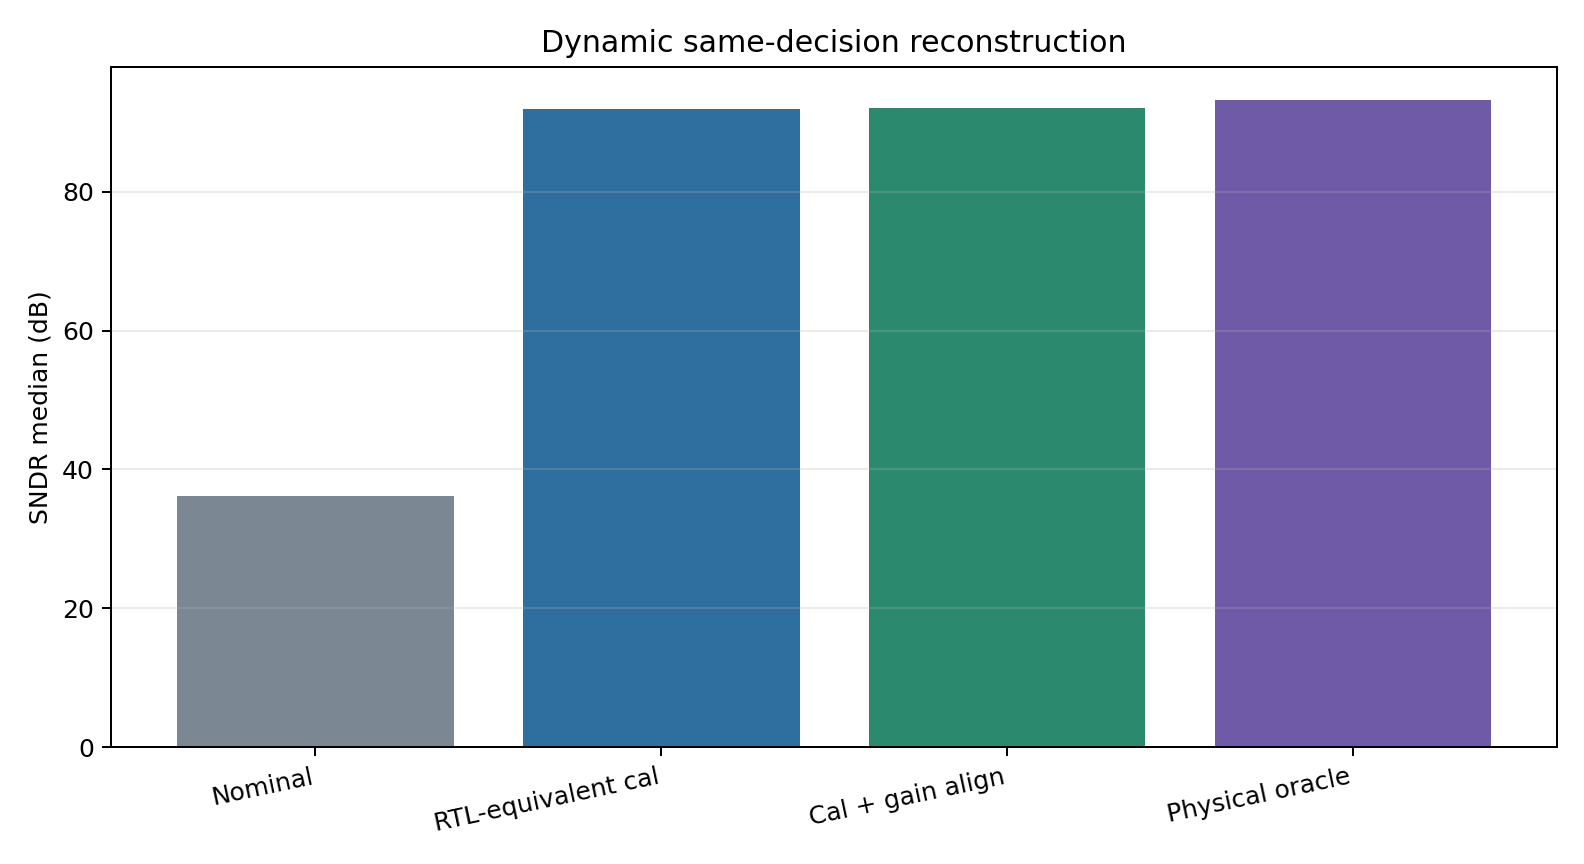
\includegraphics[width=0.86\linewidth]{../outputs/fig_dynamic_sndr_median.png}
  \caption{同一物理 decision stream 下四种解码路径的 SNDR 中位数。}
\end{figure}

\begin{figure}[htbp]
  \centering
  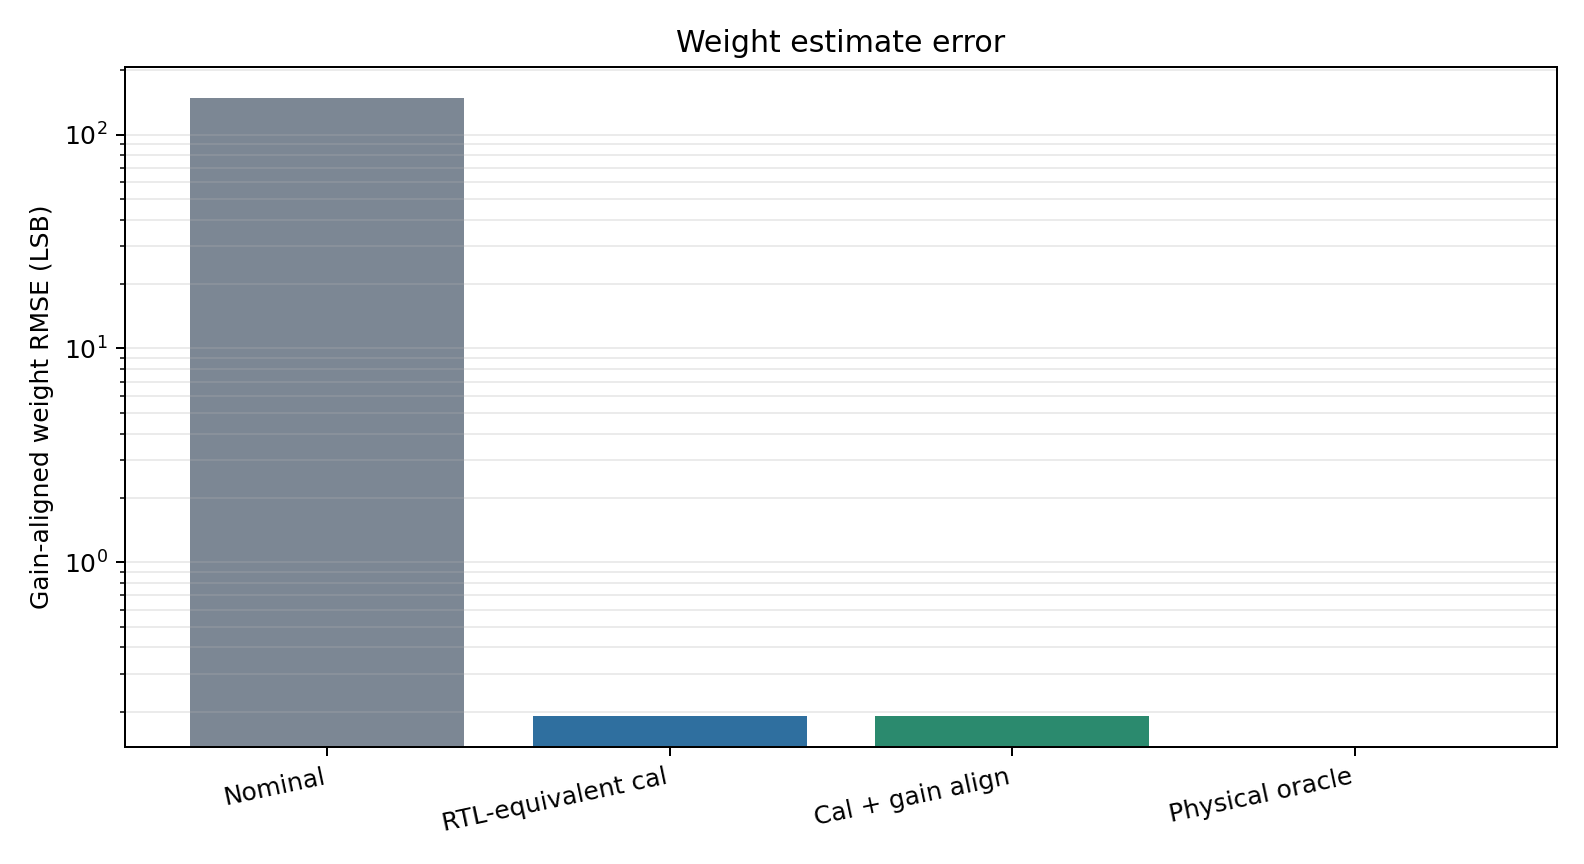
\includegraphics[width=0.86\linewidth]{../outputs/fig_weight_rmse.png}
  \caption{gain-aligned 权重 RMSE。校准后权重误差接近物理 oracle 下限。}
\end{figure}

结果表明，当前 RTL 等效校准能够显著恢复权重精度。直接使用 nominal 权重时，失配造成权重 RMSE
中位数 \NominalWeightRmseMed{} LSB，动态 SNDR 中位数 \NominalSndrMed{} dB。使用当前片上校准
权重后，gain-aligned 权重 RMSE 中位数降至 \CalGainWeightRmseMed{} LSB，动态 SNDR 中位数升至
\CalGainSndrMed{} dB。

需要注意，\texttt{RTL\_CAL\_RAW} 的动态 SNDR 已接近 \texttt{RTL\_CAL\_GAIN\_COMP}，但静态
RMS 误差仍较大。这说明当前校准控制器可以估出相对权重，而完整系统仍需要明确的全局增益归一化或
输出标尺策略。现有 \texttt{tb\_gain\_comp\_check\_lsb.sv} 也采用 MSB anchored gain compensation
进行残差评分，因此报告将该路径作为诊断而不是宣称 RTL 已包含该增益补偿寄存器。

\section{RTL 电路级验证证据}

本轮同时运行当前仓库 Vivado XSIM 回归：
\begin{itemize}
  \item \texttt{tb\_sar\_recon\_binary\_norm}: PASS，49 checks，0 failed；
  \item \texttt{tb\_recon\_q8\_split\_weights}: PASS，17 checks，0 failed；
  \item \texttt{tb\_srm\_residue\_estimator}: PASS，17 checks，0 failed；
  \item \texttt{tb\_gain\_comp\_check\_lsb}: PASS，5 Monte Carlo runs，worst residual 0.4937 LSB；
  \item XSIM overall result: PASS。
\end{itemize}

RTL 回归证明当前 SystemVerilog 可编译、可仿真，并且校准控制器、Q8 split-weight 重构契约、
binary-normalized smoke path 与 SRM LUT 单元没有退化。行为级矩阵则进一步说明，在同一物理
decision stream 约束下，当前校准算法对动态与权重误差有明确改善。

\section{与 12-bit 项目经验的差异}

12-bit 项目中的 Candidate A 验证强调三条经验：同条件批次、同决策三路解码、静态与动态分口径。
本项目吸收的是这些验证原则，而不是复制其校准算法。

关键差异如下：
\begin{itemize}
  \item 12-bit 项目使用 Candidate A 等效 CDAC 与开源 least-squares/sine calibration 评估；本项目验证的是
        \texttt{sar\_calib\_ctrl\_serial.sv} 的片上递归 P/N 搜索。
  \item 12-bit 项目强调 dual capture 与 ADCToolbox 权重识别；本项目当前片上校准不依赖外部训练音或矩阵求解。
  \item 12-bit 项目输出对称等效 CDAC 结论；本项目输出 Q8 权重写回到 \texttt{sar\_reconstruction.sv}。
  \item 两者共同要求：不能用动态 SNDR 单独替代静态 DNL/INL，也不能从行为级结果外推到硅后。
\end{itemize}

\section{工程结论与限制}

\begin{verdictbox}{Green}{可以支持的结论}
在本报告覆盖的行为级条件下，当前文件夹中的片上前台校准算法是有效的。它能把主要由高位权重失配引起的
数字重构误差大幅压低，并使动态性能接近物理权重 oracle。
\end{verdictbox}

\begin{verdictbox}{Orange}{不能支持的结论}
本报告不能证明完整 ADC 的流片级性能。尚未覆盖真实 physical CDAC charge redistribution、
sampling switch nonlinearity、reference settling、comparator ready/metastability、SRM 动态注入、
PVT、post-layout parasitics、DFT/scan、ASIC STA 和 silicon measurement。
\end{verdictbox}

建议下一步工作：
\begin{enumerate}
  \item 在 RTL 中明确是否需要全局增益归一化寄存器，避免 \texttt{RTL\_CAL\_RAW} 与 TB scoreboarding
        之间存在解释差异；
  \item 将行为级模型的 P/N 独立物理权重扩展到当前 20-bit split CDAC；
  \item 增加一个系统级 RTL/behavior co-sim，把 \texttt{w\_wr\_data} trace 与 Python 校准 trace 逐 target 对齐；
  \item 后续 AMS/Spectre 中用真实 comparator ready 替代固定 \texttt{COMP\_WAIT\_CYC} 假设。
\end{enumerate}

\section{复现路径}

\begin{enumerate}
  \item 行为级验证：\path{python analysis/calibration_effectiveness_20260729/}\\
        \path{validate_current_calibration.py}
  \item 报告资产：\path{python analysis/calibration_effectiveness_20260729/}\\
        \path{generate_report_assets.py}
  \item 进入报告目录：\path{cd analysis/calibration_effectiveness_20260729/report}
  \item 三遍编译：\path{xelatex current_calibration_validation_report_cn.tex}
  \item RTL 回归：\path{powershell -NoProfile -ExecutionPolicy Bypass -File scripts/run_all_xsim.ps1}
\end{enumerate}

行为级输出位于：
\begin{itemize}
  \item \path{analysis/calibration_effectiveness_20260729/outputs/summary.json}
  \item \path{analysis/calibration_effectiveness_20260729/outputs/per_chip_results.csv}
  \item \path{analysis/calibration_effectiveness_20260729/outputs/fig_dynamic_sndr_median.png}
  \item \path{analysis/calibration_effectiveness_20260729/outputs/fig_weight_rmse.png}
\end{itemize}

\end{document}
